\section{Проектирование программы} 
\label{sec:program_design}

Разработка программного обеспечения будет выполняться на языке C++. Выбран этот язык, так как библиотека OpenCV разработана изначально на нем. С++ позволяет разработать программы более быстродейственные, так как в процессе анализа и обработки видеопотока необходима производительность. В программе будут реализованы следующие алгоритмы обнаружения: обнаружение движений будет выполняться двумя ранее представленными методами: методом межкадровой разницы и методом вычитания фона, а обнаружение лиц методом Виолы"--~Джонса. Метод вычитания фона для обнаружения движений использует алгоритм ассоциативной модели гауссова смешения для моделирования фона. Алгоритм реализован в классе BackgroundSubtractorMOG2 библиотеки OpenCV.

\subsection{Элементы библиотеки OpenCV.}
\label{sec:program_design:opencv_elements}
Рассмотрим подробнее структуры и функции входящие в библиотеку OpenCV, необходимые для выполнения в рамках данного проекта~\cite{opencvdoc}. 

\subsubsection{Основные структуры данных. }
\label{sec:program_design:opencv_elements:ocv_structs}
Для хранения изображений в памяти используется класс Mat, представляющий собой двухмерные матрицы.

Для хранения одномерных массивов данных используется класс Scalar. В проекте используется для хранения координат цвета в цветовой модели RGB в виде массива из трех координат.

Класс Point используется для хранения информации о точке --- координаты X и Y.

\subsubsection{Работа с веб-камерой. }
\label{sec:program_design:opencv_elements:ocv_webcam}
Для получения изображения с веб"=камеры используется класс VideoCapture. Конструктор класса позволяется получить доступ к любой камере установленной в системе. Для получения доступа к основной камере конструктор запускается с параметром 0.
Для проверки подключения камеры в классе существует метод isOpened.

Для получения изображения с камеры используется оператор чтения из потока $>>$.

\subsubsection{Обработка изображений. }
\label{sec:program_design:opencv_elements:ocv_imgproc}
Для преобразования цветовой модели изображения используется функция cvtColor. В параметрах описываются входная и выходная матрицы и константа указывающая преобразование.

Функция absdiff используется для формирования изображения на основе сравнения двух других. На входе --- два изображения. На выходе --- изображение с пикселями, которые не совпадают на двух исходных образцах.

Для получения одинаковых пикселей на изображениях используется функция bitwise\_and.

Для выравнивания значений пикселей изображения по порогу используется функция threshold. На входе задаются входная и выходная матрица, пороговое значение пикселя, максимальное значение пикселя тип пороговой функции.
Значение пикселя в данном случае --- значение элемента матрицы.

Функция erode позволяет убирать шумы с изображения посредством объединения соседних пикселей в группы, задаваемые ядром --- геометрическим примитивом определенного размера. На входе задаются входное и выходное изображение и ядро.

Функция dilate выполняет операцию свертки изображения и ядра. Можно говорить что эта функция используется для расширения ярких участков изображения.

Функция resize изменяет размеры изображения.

Функция equalizeHist выравнивает гистограмму изображения, заданного в серых тонах. Алгоритм, используемый в функции, нормализует яркость и улучшает контраст изображения.

\subsubsection{Поиск контуров. }
\label{sec:program_design:opencv_elements:ocv_findcontours}
Для поиска контуров объектов на изображении используется функция findContours. Она позволяет найти контуры на одноканальном (монохромном) изображении.
На выходе функция формируем массив контуров.
Нарисовать контуры на изображении позволяет функция drawContours.

\subsubsection{Средсва рисования. }
\label{sec:program_design:opencv_elements:ocv_drawfeatures}
Для рисования на экран графических примитивов испольуются следующие функции: rectangle --- для рисования на изображение прямоугольника, circle --- для рисования круга.

Для отображения одного изображения на другом необходимо выделить на исходном изображении область в которую следует поместить другое изображение, а затем используя метод copyTo класса Mat скопировать изображение в область другого. В проекте используется для отрисовки кнопок, а также наложения контуров определяемых объектов.

\subsubsection{Поиск объектов на изображении. }
\label{sec:program_design:opencv_elements:ocv_objdetect}
Поиск объектов выполняется, используя классификатор называемый каскадом(полностью: каскад классификаторов использующих признаки Хаара).  В OpenCV за данный классификатор отвечает класс CascadeClassifier.
Метод класса load загружает готовый классификатор из файла. Метод detectMultiScale обнаруживает объекты различных размеров на входном изображении и возвращает список прямоугольников с обнаруженными объектами.

\subsubsection{Выделение фона. }
\label{sec:program_design:opencv_elements:back_subtraction}
Класс BackgroundSubtractorMOG2 отвечает за выделение фона. В конструкторе указываются конкретные параметры алгоритма, такие как порог чувствительности и количество кадров в истории, формирующих фон.
Оператор круглые скобки () добавляет кадр в историю и выделяет измененные области.

\subsubsection{Управление окнами и устройствами ввода. }
\label{sec:program_design:opencv_elements:ocv_io}
Для создания именованного окна используется функция namedWindow. Обращение к окну реализуется через имя этого окна. Функция moveWindow изменяет положение окна.
Для управления мышью в пределах окна используется функция setMouseCallback, которая при изменении событий мыши вызывает функцию заданную пользователем.
Для получения кода нажатой клавиши нужно вызвать функцию waitKey.

\subsubsection{Работа с GPU. }
\label{sec:program_design:opencv_elements:GPU}
Работа с GPU осуществоляется с использованием технологии CUDA. Класс GpuMat хранит изображения. Метод класса upload преобразует Mat в GpuMat. Для обнаружения образов через касказы Хаара используют класс CascadeClassifier\_GPU.
Работа с классами аналогична работе их CPU аналогов. 


\subsection{Компоненты приложения. }
\label{sec:program_design:components}
Диаграмма компонентов приложения представлена на рисунке~\ref{fig:components}
\begin{figure}[ht]
\centering
    \centering
    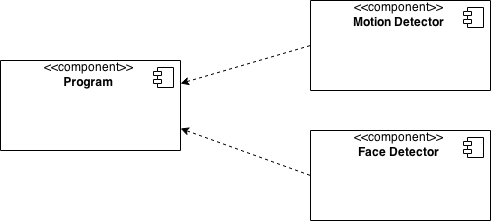
\includegraphics[scale = 0.6]{components.png}  
  \caption{Диаграмма компонентов приложения.}
  \label{fig:components}
\end{figure}

Program --- компонент реализует графический интерфейс, получение и вывод изображения, а также переключение режимов приложения. 
Компонент представлен в исходных файлах DetectionSystem.h и DetectionSystem.cpp.

MotionDetector --- компонент реализует режим обнаружения движений в приложении.
Компонент представлен в исходных файлах motiondetect.h и motiondetect.cpp.

FaceDetector --- компонент реализует режим обнаружения лиц в приложении. 

Компонент представлен в исходных файлах facedetect.h и facedetect.cpp.

Переключение между режимами в приложении реализовано в виде изменения состояния приложения.

\subsection{Блок-схемы алгоритмов. }
\label{sec:program_design:flowcharts}

\begin{figure}[ht]
\centering
    \centering
    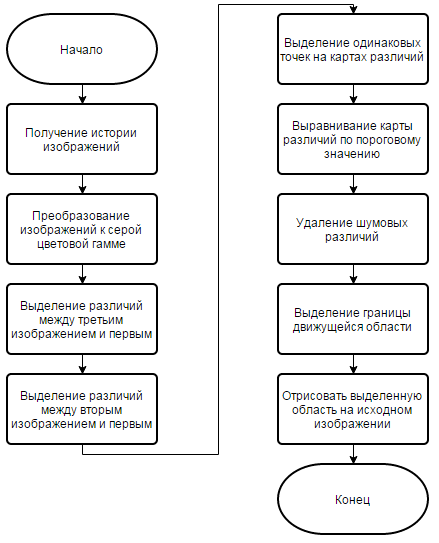
\includegraphics[scale = 1]{alg_diff.png}  
  \caption{Блок-схема алгоритма сравнения изображений.}
  \label{fig:alg_diff}
\end{figure}

\begin{figure}[ht]
\centering
    \centering
    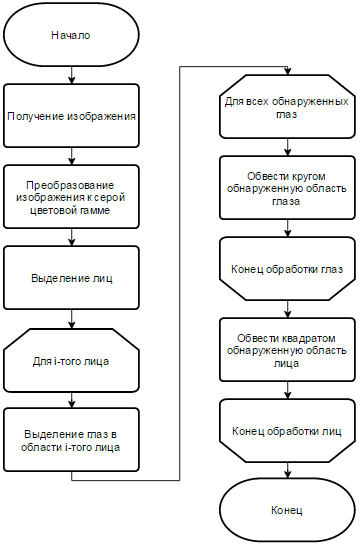
\includegraphics[scale = 1]{face_detect.png}  
  \caption{Блок-схема алгоритма выделения лиц.}
  \label{fig:alg_face}
\end{figure}
